%   Filename    : chapter_4.tex 
\chapter{Research Methodology}
This chapter lists and discusses the specific steps and activities that will be performed to accomplish the project. 
The discussion covers the activities from pre-proposal to Final SP Writing.

\section{Research Activities}
\subsection{Data Gathering} 
A dataset of sentences containing Generation Z slang and its formal translation was used in this study. 
This dataset was created using several source: data obtained from social media posts and manually translated by the researchers, existing datasets from HuggingFace, and machine generated and translated sentences using GPT-4o from OpenAI.

The data obtained from social media posts were from verified users of X whose ages are within the Generation Z, so that the dataset is accurate. The data was manually translated by the researchers to ensure that the translation is accurate and reflective of the target demographic. Data obtained from existing datasets and GPT-4o was checked manually to check if whether the sentence is one used by Generation Z. These processes ensured that the dataset is of high quality and representative of what and how Generation Z slang is used.

\subsection{Data Preprocessing} 
The dataset used for the fine-tuning of the model was preprocessed to ensure optimal performance of the model.
Unnecessary information such as email addresses and URLs was removed. The data was then manually cleaned up to remove unnecessary characters such as emojis and fixed issues such as typos. A similar approach was done with existing and machine generated datasets to ensure consistency within the training dataset.

The dataset is then split into train and test datasets in a 90/10 ratio to maximize the data learned by the model without compromising on the model's ability to generalize to new data. The train dataset is then split again into a 90/10 ratio to ensure no overfitting while still allowing the model to adapt to the pattern of slang. The cleaned up dataset was then tokenized through the Transformers library provided by HuggingFace as the library already has tokenizers available for their pretrained models.
This ensures that the data is formatted properly as required by the model to be used.

\subsection{Model Fine-Tuning}
The model used in this study was zephyr-7b-beta because it is open-source and was proven to perform better than other models of the same size. In addition, it can be trained in a GPU with 16GB of VRAM, necessary as we are using the free tier of Google Colab as the platform of choice for prototype fine-tuning of the model.

This study used the example codes provided by HuggingFace in the documentation of their various libraries and sample notebook provided in the zephyr-7b-beta repository. 

The model was loaded using the Transformers library and was quantized into 4 bits through BitsandBytes library to fit the entire model in the allocated resources while having enough headroom for training. In addition, the Unsloth library was used to speed up the training time and reduce the resources used even more \cite{unsloth}. A LoRA adapter was then attached to the model to further reduce the parameters to be trained.

To evaluate the model training process and ensure that the model is not overfitting, Bilingual Evaluation Understudy (BLEU) and Recall-Oriented Understudy for Gisting Evaluation (ROUGE) are used. BLEU is used to measure the precision of the model by determining how much of the generated text appear in the reference text \cite{papineni_roukos_ward_zhu_2001} while ROUGE is used to measure recall as it determines how much of the reference text is in the generated text \cite{lin_2004}. These metrics use n-grams, making them superior to standard recall and precision metrics as they take into account the positioning of the words. These two metrics were implemented using the Evaluate library by HuggingFace, making it easier to integrate with the rest of the model training process. These metrics was calculated at every epoch of the training process and is used for an early stopping callback to immediately stop the model training if the model seems to be overfitting.

The model was then trained using SFTTrainer from the TRL library of HuggingFace to simplify the training process. The model was trained with the following parameters: optimizer is paged 4bit AdamW, batch size of 8, learning rate of 2e-5, and maximum number of epochs of 50. These parameters were chosen based on the GPU provided in Colab, the test notebook by HuggingFace and the default parameters of SFTTrainer.

\subsection{Model Evaluation}
The model was evaluated using both automatic and manual evaluation metrics. The model was then prompted to generate a formal sentence for each sentence in the test dataset. The generated sentences were then compared to the formal translation of the sentence using BLEU and ROUGE metrics. The base zephyr-7b-beta model was also prompted to generate sentences for the BLEU and ROUGE metric and the pairwise comparison for human evaluation. Identical answers between the finetuned and the base model were removed to in the test set to ensure that the model is evaluated properly. A total of 144 sentences were used to evaluate the model.

A survey was conducted to compare the finetuned model to the base model to determine if the finetuning was effective. The survey was conducted online using Google Forms asked the participants to pick which of the following sentences is the more accurate translation of the given sentence based on accuracy, naturalness, and context. The order in which sentences from the two models were shown was randomly selected to avoid bias. To improve the response rate of the survey, the survey was split into multiple sets, answered by the same groups of people, allowing them to answer any or all of the survey forms.

\begin{figure}[H]
	\centering
	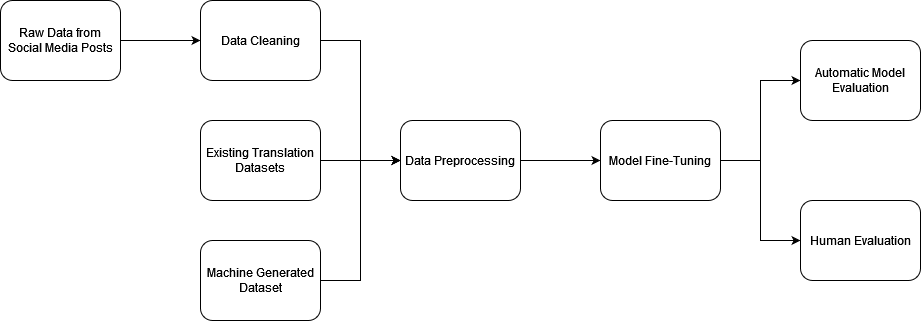
\includegraphics[scale=0.5]{figures/methodology.png}
	\caption{Summarized Methodology}
\end{figure}